\lab{Applications}{Markov Chains I}{Markov Chains I}
\label{lab:MarkovGraph}
\objective{Learn about powerful applications of linear algebra in other fields of mathematics.}

\section*{Markov Chains}
A Markov Chain describes a particular type of random process that
undergoes a sequence of transitions among various states. It is 
characterized by the fact that all relevant information is related to its current state. 
We can easily model this process using matrices.
We will start with a simple example of a frog jumping from one lily pad to another.

Suppose a frog jumps around between the three lily pads 1, 2, and 3. 
These three pads are taken as the possible \emph{states} of the system, and the
lily pad on which the frog is presently sitting is the \emph{current state}.  
If the frog is on lily pad 1 and jumps, there is a 25\% chance that it will land back on lily pad 1, a 25\% chance that it will land on lily pad 2, and a 50\% chance that it will land on lily pad 3.
We can find similar probabilities if he starts on lily pad 2 or 3.
Such probabilities are known as the \emph{transition probabilities}.
In figure \ref{fig:markov1} we have a transition diagram that reflects the various probabilities of jumping from one lily pad to another.

\begin{figure}[h]
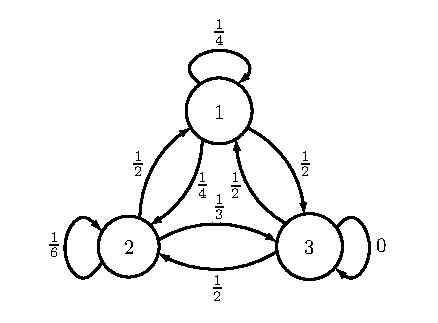
\includegraphics[width=\textwidth]{markov1}
\caption{Transition diagram for Fredo the Frog}
\label{fig:markov1}
\end{figure}

We can convert our transition diagram into a transition matrix, where the $(i,j)$-entry of the matrix corresponds to the probability that the frog jumps from the $j^{th}$ lily pad to the $i^{th}$ lily pad (where $1$ is the first lily pad, $2$ is the second, and so on).
The transition matrix is
\[
A = \begin{pmatrix}
1/4 & 1/2 & 1/2\\
1/4 & 1/6 & 1/2\\
1/2 & 1/3 & 0
\end{pmatrix}
\]
Note that all of the columns add up to one.
This is important. 

If the frog is on lily pad 1, where will it be after two jumps?
By multiplying the matrix $A$ by itself, we have (approximately)

\[
A^2 = \begin{pmatrix}
0.4375 & 0.3750 & 0.3750\\
0.3542 & 0.3194 & 0.2083\\
0.2083 & 0.3056 & 0.4167
\end{pmatrix}
\]
From this, we infer that there is a 43.75\% chance the frog will still be on lily pad 1 after two jumps.
Note that it might have jumped from 1 to 1 to 1, denoted $1 \rightarrow 1 \rightarrow 1$, or it could have jumped to one of the other lily pads and then back again, that is, either $1 \rightarrow 2 \rightarrow 1$ or $1 \rightarrow 3 \rightarrow 1$.
In addition, there is a 35.42\% chance it will be on lily pad 2 and a 20.83\% chance that it will be on lily pad 3.
Using Python, we can type in our transition matrix and see where the frog will be after 5, 10, 20 or 100 jumps.

\begin{lstlisting}
#Remember, the 1.'s in the numerator force floating point division
>>> A = np.array([[1./4,1./2,1./2],[1./4,1./6,1./2],[1./2,1./3,0]])
>>> np.linalg.matrix_power(A,5)
>>> np.linalg.matrix_power(A,10)
>>> np.linalg.matrix_power(A,20)
>>> np.linalg.matrix_power(A,100)
\end{lstlisting}

Note that as we take higher powers it appears that the limit goes to
\[
A^\infty = \begin{pmatrix}
0.4 & 0.4 & 0.4\\
0.3 & 0.3 & 0.3\\
0.3 & 0.3 & 0.3
\end{pmatrix},
\]
and this can, in fact, be proven carefully.
This means that after several jumps, the probability that we will find Fredo on a given lily pad will have nothing to do with where he started initially.


We can generalize this notion beyond that of frogs and lily pads.
Let the state distribution of our system be represented by a probability vector
\[
\x = \begin{bmatrix}
x_1\\
x_2\\
\vdots\\
x_n
\end{bmatrix}
\]
where each entry represents the probability of being in that state.
Note that each entry is non-negative and the sum of all the entries adds up to one.
For example, in the frog example, if we know initially that it is on lily pad 1, then we have the probability vector
\[
\x_0 = \begin{bmatrix}
1\\
0\\
0
\end{bmatrix}
\]
because we know for certainty (100\%) that the frog is in the first state.
After one jump, we have
\[
\x_1 = A \x_0 = \begin{bmatrix}
0.25\\
0.25\\
0.50
\end{bmatrix}
\]
After two jumps, we have
\[
\x_2 = A \x_1 = A^2 \x_0 = \begin{bmatrix}
0.4375\\
0.3542\\
0.2083
\end{bmatrix}
\]
After a large number of jumps $(n>>1)$, we have
\[
\x_n = A \x_{n-1} = \dots = A^n \x_0 \approx \begin{bmatrix}
0.4\\
0.3\\
0.3
\end{bmatrix}
\]
Since all of the columns are the same for $A^\infty$, it follows that for any initial probability vector $\x_0$, we get the same limiting output, or in other words, all initial vectors converge to the same point, call it $\x_\infty$.
Moreover, we have that
\[
\x_\infty = A \x_\infty
\]
This is called a \emph{stable fixed point}.
How can we check that a stable fixed point exists?
We can investigate these matters further using a couple of tools from 
linear algebra and matrix theory, namely eigenvalues and eigenvectors.

\section*{Example}
Consider the Markov chain given by
\[
A = \begin{pmatrix}
0.5 & 0.3 & 0.4\\
0.2 & 0.2 & 0.3\\
0.3 & 0.5 & 0.3
\end{pmatrix}.
\]
We show that it has a stable fixed point by checking that it has a single eigenvalue $\lambda=1$.
We do this via Python:
\begin{lstlisting}
>>> from scipy import linalg as la
>>> A = np.array([[.5,.3,.4],[.2,.2,.3],[.3,.5,.3]])
>>> V = la.eig(A)[1]
\end{lstlisting}
Note that the entries in the $\lambda=1$ eigenvector do not generally add up to one.
Indeed, any multiple of an eigenvector is an eigenvector.
So we need to multiply it by the appropriate constant so that all of the entries add up to one.
\begin{lstlisting}
>>> x = V[:,0]
>>> x = x/sp.sum(x);x
array([ 0.41836735,  0.23469388,  0.34693878])
\end{lstlisting}
We can check this answer by taking $A$ to a high exponent, say $A^{100}$.

\begin{problem}
Suppose a basketball player's success at shooting free throws can be described with the following Markov chain
\[
A = \begin{pmatrix}.75&.50\\.25&.50\end{pmatrix}
\]
where the first state corresponds to success and the second state to failure.
\begin{enumerate}
\item If the player makes his first free throw, what is the probability that he also makes his third one?
\item What is the player's average free throw percentage?
\end{enumerate}
\end{problem}

\begin{problem}
Consider the Markov process given by the transition diagram in Figure \ref{fig:markov2}.
\begin{figure}[H]
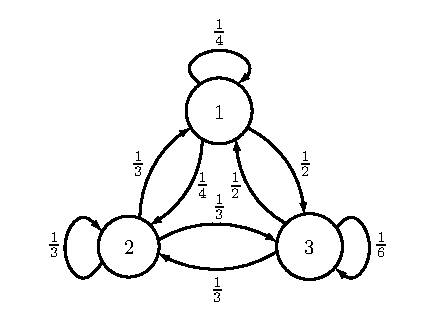
\includegraphics[width=\textwidth]{markov2}
\caption{Transition diagram}
\label{fig:markov2}
\end{figure}

\begin{enumerate}
\item Find the transition matrix.
\item If the Markov process is in state 1 initially, find the probability that it is in state 2 after 2 transitions.
\item Find the stable fixed point if it exists.
\end{enumerate}
\end{problem}

\section*{Uses in Graph Theory}
\begin{figure}[h]
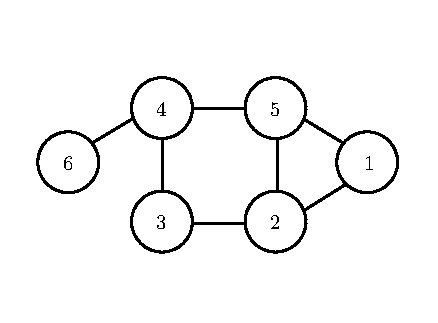
\includegraphics[width=\textwidth/2]{graphExample}
\caption{A simple graph}
\label{fig:example_graph}
\end{figure}

Graphs are often used to represent relationships between objects.
They are represented by a set of nodes (or vertices) and a set of edges where each edge connects exactly two nodes.
A graph is \emph{directed} if connections are uni-directional, and \emph{undirected} if they are bi-directional.
Every undirected edge can be represented as two directed edges.
Figure \ref{fig:example_graph} shows a simple undirected graph.
We can represent the connections of nodes as a matrix called an \emph{adjacency matrix}.
The graph in Figure \ref{fig:example_graph} can be represented as the following adjacency matrix.
\[
A = \begin{pmatrix}
0 & 1 & 0 & 0 & 1 & 0\\
1 & 0 & 1 & 0 & 1 & 0\\
0 & 1 & 0 & 1 & 0 & 0\\
0 & 0 & 1 & 0 & 1 & 1\\
1 & 1 & 0 & 1 & 0 & 0\\
0 & 0 & 0 & 1 & 0 & 0
\end{pmatrix}
\]
We order the nodes and each node represents one column and one row of the adjacency matrix.
If an edge exists between node $i$ and node $j$ then the $A_{ij}$ entry is 1.
For undirected graphs, the adjacency matrix will always be symmetric.
The diagonal represents self-edges, or edges that connect a node to itself.
While adjacency matrices are useful, many graph algorithms depend on another representation of a graph called an \emph{adjacency list}.

Raising the adjacency matrix to a power yields some very interesting information.
We can discover the number of paths of length $n$ between to nodes by raising a graph's adjacency matrix to the $n$th power.
For example, by squaring $A$, we can find the number of paths of length 2 between every pair of nodes. 
\begin{lstlisting}
>>> np.linalg.matrix_power(A,2)
array([[2, 1, 1, 1, 1, 0],
       [1, 3, 0, 2, 1, 0],
       [1, 0, 2, 0, 2, 1],
       [1, 2, 0, 3, 0, 0],
       [1, 1, 2, 0, 3, 1],
       [0, 0, 1, 0, 1, 1]])
\end{lstlisting}
We can see that no paths of length 2 exist between node 0 and node 5 because $A^2_{0,5} = 0$.
By calculating $A^6$ we can find the number of paths length 6 from node 3 to itself.
\begin{lstlisting}
>>> np.linalg.matrix_power(A, 6)
array([[45, 54, 38, 45, 54, 16],
       [54, 86, 29, 77, 51, 11],
       [38, 29, 55, 15, 70, 27],
       [45, 77, 15, 75, 31,  4],
       [54, 51, 70, 31, 93, 34],
       [16, 11, 27,  4, 34, 14]])
\end{lstlisting}
We see that there are 55 unique paths of length 6 from node 3 to itself.
Imagine trying to count all of those paths by hand!
It would be very easy to count incorrectly.
However, this method makes it very simple to count paths without any mistakes.

Adjacency matrices can also be composed of \li{True} and \li{False} values.
In this case, the $n$th power of such a matrix (using boolean arithmetic)
is again a matrix of
boolean values which simply indicate whether there exists a path of length $n$ between the given pair of nodes, rather than indicating the number of such
paths.

\begin{problem}
Let the following matrix represent a directed graph
\[
\begin{pmatrix}
0 & 0 & 1 & 0 & 1 & 0 & 1 \\
1 & 0 & 0 & 0 & 0 & 1 & 0 \\
0 & 0 & 0 & 0 & 0 & 1 & 0 \\
1 & 0 & 0 & 0 & 1 & 0 & 0 \\
0 & 0 & 0 & 1 & 0 & 0 & 0 \\
0 & 0 & 1 & 0 & 0 & 0 & 1 \\
0 & 1 & 0 & 0 & 0 & 0 & 0
\end{pmatrix}
\]
Between which pair of nodes does there exist the greatest number of paths
of length five?
From which node to which node is there no path of length seven?
\end{problem}

Another useful way of representing an undirected graph is a Laplacian matrix.
This special matrix can reveal a lot of information about a graph.
\begin{definition}
For a simple graph (an unweighted, undirected graph without self-edges), the Laplacian of a graph $G$ is
\[ L_G = D_G - A_G \]
where $D_G$ is the degree matrix of $G$ and $A_G$ is the adjacency matrix of $G$.
\end{definition}
An important question in working with graphs is the degree of its nodes.
The degree of a node is how many edges connect to a node.  
For a directed graph, each node has an \emph{out-degree} (the number of edges directed away from a node) and an \emph{in-degree} (the number edges directed toward a node).
The degree matrix of a graph is a diagonal matrix that has the degree of each node as the diagonal entries.

\begin{problem}
Calculate the Laplacian matrix of the graph in Figure \ref{fig:example_graph} by calculating $D$ and $A$.
Think about how to find the number of neighboring nodes using an adjacency matrix.

Write a general solution that will calculate the Laplacian of any small graph.
Use the adjacency matrix to check that the graph is unweighted, undirected, and contains no self-edges.
\label{prob:laplacian}
\end{problem}
